
\documentclass[conference]{IEEEtran}

\IEEEoverridecommandlockouts 
% this is needed to allow the \IEEEpubid command used to add the copyright
% notice at the bottom of the first page. 
% See  How_to_add_Copyright_in_LaTeX_file.txt  for more info

% *** MISC UTILITY PACKAGES ***
%
% \usepackage{ifpdf}
% Heiko Oberdiek's ifpdf.sty is very useful if you need conditional
% compilation based on whether the output is pdf or dvi.
% usage:
% \ifpdf
%   % pdf code
% \else
%   % dvi code
% \fi
% The latest version of ifpdf.sty can be obtained from:
% http://www.ctan.org/tex-archive/macros/latex/contrib/oberdiek/
% Also, note that IEEEtran.cls V1.7 and later provides a builtin
% \ifCLASSINFOpdf conditional that works the same way.
% When switching from latex to pdflatex and vice-versa, the compiler may
% have to be run twice to clear warning/error messages.

% *** CITATION PACKAGES ***
%
%\usepackage{cite}
% cite.sty was written by Donald Arseneau
% V1.6 and later of IEEEtran pre-defines the format of the cite.sty package
% \cite{} output to follow that of IEEE. Loading the cite package will
% result in citation numbers being automatically sorted and properly
% "compressed/ranged". e.g., [1], [9], [2], [7], [5], [6] without using
% cite.sty will become [1], [2], [5]--[7], [9] using cite.sty. cite.sty's
% \cite will automatically add leading space, if needed. Use cite.sty's
% noadjust option (cite.sty V3.8 and later) if you want to turn this off.
% cite.sty is already installed on most LaTeX systems. Be sure and use
% version 4.0 (2003-05-27) and later if using hyperref.sty. cite.sty does
% not currently provide for hyperlinked citations.
% The latest version can be obtained at:
% http://www.ctan.org/tex-archive/macros/latex/contrib/cite/
% The documentation is contained in the cite.sty file itself.
\usepackage{mathptmx,graphicx}
\DeclareGraphicsExtensions{.pdf,.png}

% *** GRAPHICS RELATED PACKAGES ***
%
%\ifCLASSINFOpdf
%\usepackage[pdftex]{graphicx}
  % declare the path(s) where your graphic files are
  % \graphicspath{{../pdf/}{../jpeg/}}
  % and their extensions so you won't have to specify these with
  % every instance of \includegraphics
%\DeclareGraphicsExtensions{.pdf,.png,.jpeg}
%\else
  % or other class option (dvipsone, dvipdf, if not using dvips). graphicx
  % will default to the driver specified in the system graphics.cfg if no
  % driver is specified.
%\usepackage[dvips]{graphicx}
  % declare the path(s) where your graphic files are
  % \graphicspath{{../eps/}}
  % and their extensions so you won't have to specify these with
  % every instance of \includegraphics
%\DeclareGraphicsExtensions{.eps}
%\fi
% graphicx was written by David Carlisle and Sebastian Rahtz. It is
% required if you want graphics, photos, etc. graphicx.sty is already
% installed on most LaTeX systems. The latest version and documentation can
% be obtained at: 
% http://www.ctan.org/tex-archive/macros/latex/required/graphics/
% Another good source of documentation is "Using Imported Graphics in
% LaTeX2e" by Keith Reckdahl which can be found as epslatex.ps or
% epslatex.pdf at: http://www.ctan.org/tex-archive/info/
%
% latex, and pdflatex in dvi mode, support graphics in encapsulated
% postscript (.eps) format. pdflatex in pdf mode supports graphics
% in .pdf, .jpeg, .png and .mps (metapost) formats. Users should ensure
% that all non-photo figures use a vector format (.eps, .pdf, .mps) and
% not a bitmapped formats (.jpeg, .png). IEEE frowns on bitmapped formats
% which can result in "jaggedy"/blurry rendering of lines and letters as
% well as large increases in file sizes.
%
% You can find documentation about the pdfTeX application at:
% http://www.tug.org/applications/pdftex





% *** MATH PACKAGES ***
%
\usepackage[cmex10]{amsmath}
% A popular package from the American Mathematical Society that provides
% many useful and powerful commands for dealing with mathematics. If using
% it, be sure to load this package with the cmex10 option to ensure that
% only type 1 fonts will utilized at all point sizes. Without this option,
% it is possible that some math symbols, particularly those within
% footnotes, will be rendered in bitmap form which will result in a
% document that can not be IEEE Xplore compliant!
%
% Also, note that the amsmath package sets \interdisplaylinepenalty to 10000
% thus preventing page breaks from occurring within multiline equations. Use:
\interdisplaylinepenalty=2500
% after loading amsmath to restore such page breaks as IEEEtran.cls normally
% does. amsmath.sty is already installed on most LaTeX systems. The latest
% version and documentation can be obtained at:
% http://www.ctan.org/tex-archive/macros/latex/required/amslatex/math/





% *** SPECIALIZED LIST PACKAGES ***
%
%\usepackage{algorithmic}
% algorithmic.sty was written by Peter Williams and Rogerio Brito.
% This package provides an algorithmic environment fo describing algorithms.
% You can use the algorithmic environment in-text or within a figure
% environment to provide for a floating algorithm. Do NOT use the algorithm
% floating environment provided by algorithm.sty (by the same authors) or
% algorithm2e.sty (by Christophe Fiorio) as IEEE does not use dedicated
% algorithm float types and packages that provide these will not provide
% correct IEEE style captions. The latest version and documentation of
% algorithmic.sty can be obtained at:
% http://www.ctan.org/tex-archive/macros/latex/contrib/algorithms/
% There is also a support site at:
% http://algorithms.berlios.de/index.html
% Also of interest may be the (relatively newer and more customizable)
% algorithmicx.sty package by Szasz Janos:
% http://www.ctan.org/tex-archive/macros/latex/contrib/algorithmicx/




% *** ALIGNMENT PACKAGES ***
%
\usepackage{array}
% Frank Mittelbach's and David Carlisle's array.sty patches and improves
% the standard LaTeX2e array and tabular environments to provide better
% appearance and additional user controls. As the default LaTeX2e table
% generation code is lacking to the point of almost being broken with
% respect to the quality of the end results, all users are strongly
% advised to use an enhanced (at the very least that provided by array.sty)
% set of table tools. array.sty is already installed on most systems. The
% latest version and documentation can be obtained at:
% http://www.ctan.org/tex-archive/macros/latex/required/tools/


%\usepackage{mdwmath}
%\usepackage{mdwtab}
% Also highly recommended is Mark Wooding's extremely powerful MDW tools,
% especially mdwmath.sty and mdwtab.sty which are used to format equations
% and tables, respectively. The MDWtools set is already installed on most
% LaTeX systems. The lastest version and documentation is available at:
% http://www.ctan.org/tex-archive/macros/latex/contrib/mdwtools/


% IEEEtran contains the IEEEeqnarray family of commands that can be used to
% generate multiline equations as well as matrices, tables, etc., of high
% quality.


%\usepackage{eqparbox}
% Also of notable interest is Scott Pakin's eqparbox package for creating
% (automatically sized) equal width boxes - aka "natural width parboxes".
% Available at:
% http://www.ctan.org/tex-archive/macros/latex/contrib/eqparbox/





% *** SUBFIGURE PACKAGES ***
%\usepackage[tight,footnotesize]{subfigure}
% subfigure.sty was written by Steven Douglas Cochran. This package makes it
% easy to put subfigures in your figures. e.g., "Figure 1a and 1b". For IEEE
% work, it is a good idea to load it with the tight package option to reduce
% the amount of white space around the subfigures. subfigure.sty is already
% installed on most LaTeX systems. The latest version and documentation can
% be obtained at:
% http://www.ctan.org/tex-archive/obsolete/macros/latex/contrib/subfigure/
% subfigure.sty has been superceeded by subfig.sty.



%\usepackage[caption=false]{caption}
%\usepackage[font=footnotesize]{subfig}
% subfig.sty, also written by Steven Douglas Cochran, is the modern
% replacement for subfigure.sty. However, subfig.sty requires and
% automatically loads Axel Sommerfeldt's caption.sty which will override
% IEEEtran.cls handling of captions and this will result in nonIEEE style
% figure/table captions. To prevent this problem, be sure and preload
% caption.sty with its "caption=false" package option. This is will preserve
% IEEEtran.cls handing of captions. Version 1.3 (2005/06/28) and later 
% (recommended due to many improvements over 1.2) of subfig.sty supports
% the caption=false option directly:
%\usepackage[caption=false,font=footnotesize]{subfig}
%
% The latest version and documentation can be obtained at:
% http://www.ctan.org/tex-archive/macros/latex/contrib/subfig/
% The latest version and documentation of caption.sty can be obtained at:
% http://www.ctan.org/tex-archive/macros/latex/contrib/caption/




% *** FLOAT PACKAGES ***
%
%\usepackage{fixltx2e}
% fixltx2e, the successor to the earlier fix2col.sty, was written by
% Frank Mittelbach and David Carlisle. This package corrects a few problems
% in the LaTeX2e kernel, the most notable of which is that in current
% LaTeX2e releases, the ordering of single and double column floats is not
% guaranteed to be preserved. Thus, an unpatched LaTeX2e can allow a
% single column figure to be placed prior to an earlier double column
% figure. The latest version and documentation can be found at:
% http://www.ctan.org/tex-archive/macros/latex/base/



%\usepackage{stfloats}
% stfloats.sty was written by Sigitas Tolusis. This package gives LaTeX2e
% the ability to do double column floats at the bottom of the page as well
% as the top. (e.g., "\begin{figure*}[!b]" is not normally possible in
% LaTeX2e). It also provides a command:
%\fnbelowfloat
% to enable the placement of footnotes below bottom floats (the standard
% LaTeX2e kernel puts them above bottom floats). This is an invasive package
% which rewrites many portions of the LaTeX2e float routines. It may not work
% with other packages that modify the LaTeX2e float routines. The latest
% version and documentation can be obtained at:
% http://www.ctan.org/tex-archive/macros/latex/contrib/sttools/
% Documentation is contained in the stfloats.sty comments as well as in the
% presfull.pdf file. Do not use the stfloats baselinefloat ability as IEEE
% does not allow \baselineskip to stretch. Authors submitting work to the
% IEEE should note that IEEE rarely uses double column equations and
% that authors should try to avoid such use. Do not be tempted to use the
% cuted.sty or midfloat.sty packages (also by Sigitas Tolusis) as IEEE does
% not format its papers in such ways.





% *** PDF, URL AND HYPERLINK PACKAGES ***
%
%\usepackage{url}
% url.sty was written by Donald Arseneau. It provides better support for
% handling and breaking URLs. url.sty is already installed on most LaTeX
% systems. The latest version can be obtained at:
% http://www.ctan.org/tex-archive/macros/latex/contrib/misc/
% Read the url.sty source comments for usage information. Basically,
% \url{my_url_here}.





% *** Do not adjust lengths that control margins, column widths, etc. ***
% *** Do not use packages that alter fonts (such as pslatex).         ***
% There should be no need to do such things with IEEEtran.cls V1.6 and later.
% (Unless specifically asked to do so by the journal or conference you plan
% to submit to, of course. )


% correct bad hyphenation here
\hyphenation{op-tical net-works semi-conduc-tor trans-former core-less}


\begin{document}
%
% paper title
% can use linebreaks \\ within to get better formatting as desired
\title{A modular ADC system for power data \\acquisition utilising coreless PCB transformers \\for power and signal isolation}


% author names and affiliations
% use a multiple column layout for up to three different
% affiliations
\author{\IEEEauthorblockN{Michael Carpenter and Mark A. H. Broadmeadow}
\IEEEauthorblockA{School of Electrical Engineering and Computer Science\\
Queensland University of Technology\\
Brisbane, Australia\\
Email: michael.carpenter@student.qut.edu.au}}

% conference papers do not typically use \thanks and this command
% is locked out in conference mode. If really needed, such as for
% the acknowledgment of grants, issue a \IEEEoverridecommandlockouts
% after \documentclass

% use for special paper notices
%\IEEEspecialpapernotice{(Invited Paper)}

% this creates the copyright notice at bottom of first page as required for IEEE

% MAHB - No copyright for AUPEC
%\IEEEpubid{978--1--4799--5776--7/14/\$31.00~\copyright~2014~IEEE}

% make the title area
\maketitle

\begin{abstract}
%\boldmath
Energy monitoring and power quality analysis plays a vital role in industrial and commercial situations, where data may be used to detect faults, monitor energy usage, and refine processes.  Currently, energy metering devices are typically expensive and low-bandwidth, making them poorly suited to a modular multi-sensor data collection scheme.  This paper presents the concept of a isolated, low-cost, modular data acquisition module for use in a distributed multi-sensor, single-host environment.  The paper focusses primarily on the practical use of planar coreless PCB transformers, which facilitates the module's isolated power, clock and data signal transfer.
\end{abstract}


\IEEEpeerreviewmaketitle

\section{Introduction}

Currently, industrial energy users are limited to the use of generally expensive and low-bandwidth energy usage data collection devices. Although such metering devices are well suited to high-accuracy, high-energy systems, they are poorly suited to highly modular, multi-sensor data collection schemes.  To facilitate industrial process refinement, fault detection and energy usage analysis, the Queensland University of Technology researchers are currently developing a galvanically isolated, low-cost, high-bandwidth data acquisition module. 

% MAHB: Need more context setting content in the intro + one short paragraph summarising the content of this paper
% Possible things to discuss:	Analog signal isolation....

\section{Proposed modular data acquisition system}
% MAHB: Introduce the structure of the DAQ system here
% Present the overall system but also draw out the proposed functions for the PCB transformer here to present a clear throughline into the subsequent sections wehre you discuss the implementation of each function.

% MAHB: Note that ``double quotes'' are used like this <===
The complete system (\figurename{1}) comprises of one or more data acquisition modules (herein referred to as DAQMs), a data consolidation FPGA, and a microcontroller attached to a PC, display or storage device.  
The DAQM's data conversion device is commercial dual-input sigma-delta IC, with appropriate signal conditioning to facilitate voltage measurement via a resistor divider, and current measurement via a resistive shunt or current transformer (CT).  This paper will refer to the data conversion side of the DAQM as the ``secondary'' side.  To power the sigma-delta converter and to transmit data from it to the host, as well as simultaneously providing the converter with a clock signal from the host, a single planar coreless PCB transformer is used.  For current sigma-delta converter, the clock is approximately 8MHz, with the data rate of $ f_{clock}/4 $ (voltage and current share one data stream) with the maximum input sampling rate of $ f_{clock}/12 $.
This transformer, along with the methods used to transfer power, clock and data signals, will be the focus of this paper.  The secondary side of the DAQM consists of the coreless transformer driver, clock encoding and data recovery circuitry.  

% MAHB: Note is IEEE referencing style it is not necessary to cite author names. In a few places throughout you can replace with "Presented in [1]", for example.
Planar coreless PCB transformers are not a new concept, and considerable work has been presented by Hui, et al \cite{TangHuiFundamental}.  Such papers are primarily focussed on the application of coreless PCB transformers in relatively low-frequency isolated gate drive circuits, and do not discuss high-frequency signal transfer nor bidirectional (clock and data) signal transfer whilst simultaneously extracting power from the PCB transformer's secondary planar winding.

\begin{figure}[t]
	\centering
	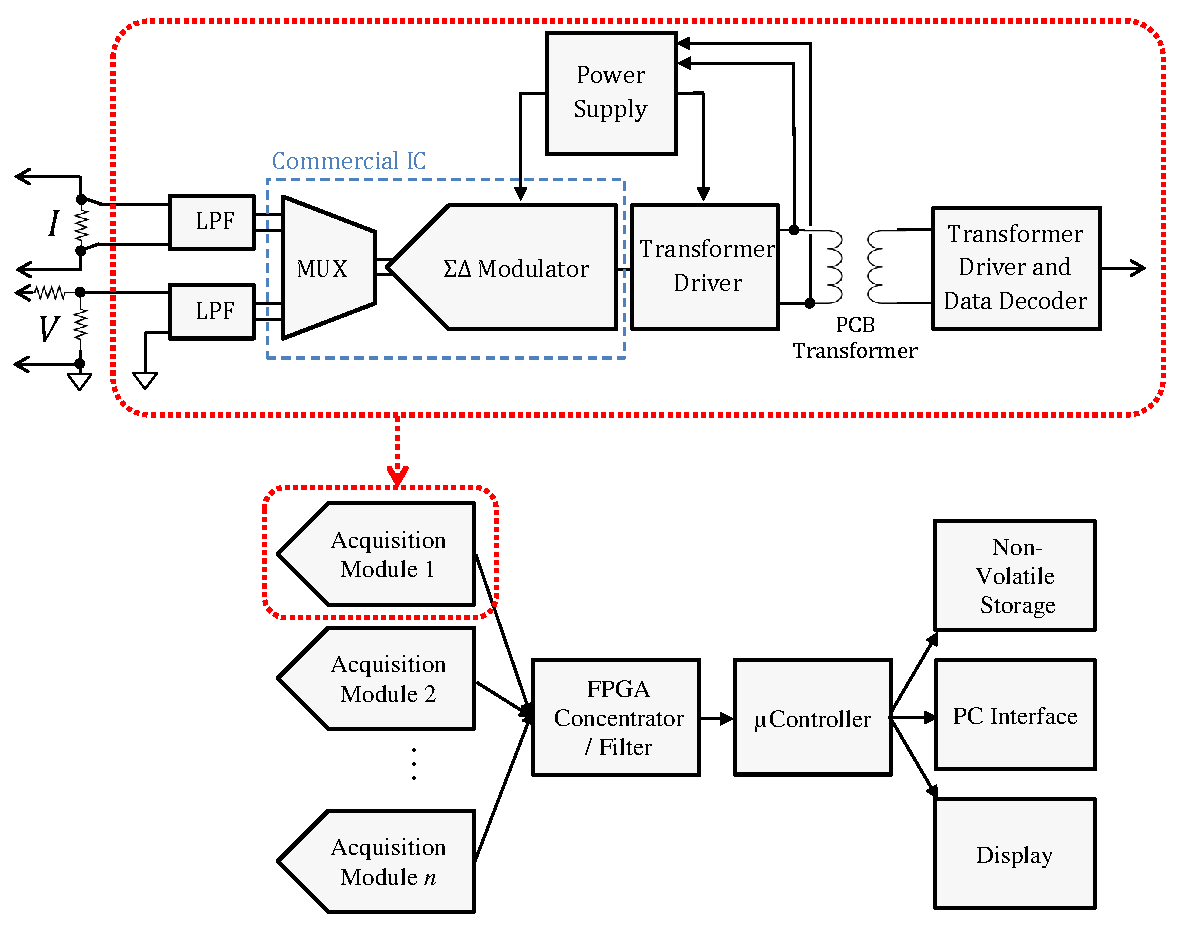
\includegraphics[width=1\columnwidth]{./img/FullSystem_BasicCol}
	\caption{Modular isolated power measurement system.}
	\label{fig:FullSystem}
\end{figure}

% MAHB: Sentence case for section headings
\section{Planar coreless PCB transformers}

The fundamental design of a planar coreless PCB transformer involves two planar copper spirals - one etched onto either side of a regular two-layer PCB.  The two windings are thus separated by the PCB's core material, whose material properties and thickness determine, to some extent, the transformer's performance and primary-to-secondary isolation.  This transformer's primary winding is then driven at high frequency, usually in the range of 2MHz to 20MHz in order to achieve either the maximum [input] impedance frequency (MIF - useful in low power systems) or the maximum efficiency frequency (MEF - useful for high power systems).  Hui, et al \cite{TangHuiFundamental} have demonstrated that an external secondary load capacitor, in the order of 100pF to 1nF, plays a significant role in the determination of the transformer's resonant frequency.  In conventional coreless PCB transformer applications, the output (ie: secondary winding) voltage is then rectified and filtered.  Transformer efficiencies exceeding 90\%, with power density of up to $ 24W/cm^{2} $ have been demonstrated \cite{TangHuiFundamental}.

Planar coreless PCB transformers are very low cost and feature high power densities, no manufacturing restrictions due to core size or shape and are constructed using highly repeatable standard PCB manufacturing process. 

\begin{figure}[t]
	\centering
	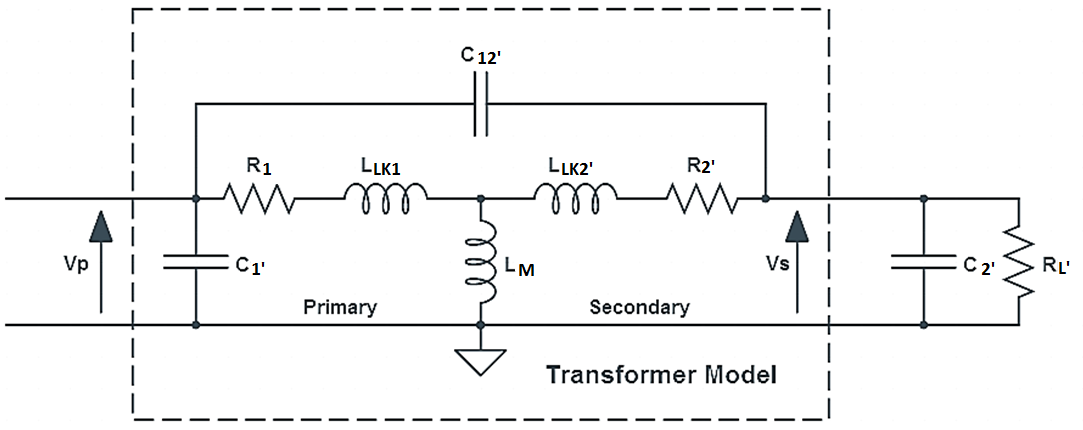
\includegraphics[width=1\columnwidth]{./img/HF_Model}
	\caption{High-frequency transformer model \cite{TangHuiFundamental}.}
	\label{fig:HF-Model}
\end{figure}

% MAHB: Prefer use of \ref{} for figure referencing as it gives control of what form of name to use: figure, fig. etc.
A two-winding coreless PCB transformer may be described using the high-frequency transformer model in figure \ref{fig:HF-Model} \cite{TangHuiFundamental}, where:
% MC: Would be good if this list was tabbed and aligned niceley.  When description goes onto two lines it looks a bit ugly
\\$ R_{1}    $ \hspace{20pt} Primary winding resistance;
\\$ R_{2}'   $ \hspace{20pt} Secondary winding resistance, referred to primary;
\\$ R_{L}'   $ \hspace{20pt} Load resistance, referred to primary;
\\$ L_{LK1}  $ \hspace{12pt} Primary leakage inductance;
\\$ L_{LK2}' $ \hspace{12pt} Secondary leakage inductance, referred to primary;
\\$ L_{M}    $ \hspace{20pt} Mutual inductance;
\\$ C_{12}   $ \hspace{19pt} Primary-to-secondary winding capacitance;
\\$ C_{1}    $ \hspace{20pt} Sum of primary winding capacitance and primary driver output capacitance;
\\$ C_{2}'   $ \hspace{20pt} Sum of secondary winding capacitance and external load capacitance, referred to primary;
\\$ n        $ \hspace{25pt} Turns ratio;
\\$ \mu_{0}  $ \hspace{20pt} Permeability of vacuum;
\\$ a_{1}    $ \hspace{20pt} Inner radius of $i$th circular track filament;
\\$ a_{2}    $ \hspace{20pt} Outer radius of $i$th circular track filament;
\\$ h_{1}    $ \hspace{20pt} Height of $i$th circular track filament;
\\$ r_{1}    $ \hspace{20pt} Inner radius of $j$th circular track filament;
\\$ r_{2}    $ \hspace{20pt} Outer radius of $j$th circular track filament;
\\$ h_{2}    $ \hspace{20pt} Height of $j$th circular track filament;
\\$ z        $ \hspace{26pt} Separation distance between the circular tracks;
\\$ J_{0}(x) $ \hspace{9pt}  Bessel function of the first kind, order zero.

\hspace{-20pt} The self inductance of the planar winding is given by
% PRI
\begin{equation}
	L_{p} = \sum\limits_{j=1}^{N_{p}}{\sum\limits_{i=1}^{N_{p}}{M_{ij}}}
\end{equation}
%
% SEC
\begin{equation}
	L_{s} = \sum\limits_{j=1}^{N_{s}}{\sum\limits_{i=1}^{N_{s}}{M_{ij}}}
\end{equation}

\hspace{-20pt} And thus, the mutual inductance between the two planar windings may be represented as
%
\begin{equation}
	M_{ps} = \sum\limits_{j=1}^{N_{p}}{\sum\limits_{i=1}^{N_{s}}{M_{ij}}}
\end{equation}

% MAHB: Removed autor names
\hspace{-20pt} where the mutual inductance, $ M_{ij} $, has been reported in \cite{HurleyDuffy}
% MAHB: Split equation over multiple lines
\begin{equation}
\begin{split}
	M_{ij} = \frac{\mu_{0}\pi}{h_{1}\ln(\frac{r_{2}}{r_{1}})h_{2}\ln(\frac{a_{2}}{a_{1}})}\int\limits_{0}^{\infty} & S(kr_{2},kr_{1})S(ka_{2},ka_{1}) 
	\\ &\quad {Q(kh_{1},kh_{2})e^{-k|z|}dk}
\end{split}
\end{equation}

\hspace{-20pt} where
\begin{equation}
	S(kx, ky) = \frac{J_{0}(kx) - J_{0}(ky)}{k}
\end{equation}
%
\begin{equation}
	Q(kx, ky) = \left\{
		\begin{array}{lr}
		\frac{2}{k^{2}} \left[ \cosh{k\frac{x+y}{2}}-\cosh{k\frac{x-y}{2}} \right] & z>\frac{h_{1}+h_{2}}{2} \\
		\frac{2}{k} \left[ h+\frac{e^{-kh}-1}{k} \right] & z=0, x=y=h
		\end{array}
   \right.
\end{equation}

\hspace{-20pt} To approximate the performance of the coreless PCB transformer, \cite{TangHuiFundamental} gives the resonant frequency as

\begin{equation}
	f_{0} = \frac{1}{2\pi\sqrt{L_{eq}C_{eq}}};
\end{equation}

\hspace{-20pt} and the $s$-domain voltage gain (\ref{eqn:vGain}) and input impedance (\ref{eqn:zIn}) of as
%
\begin{equation}
	\label{eqn:vGain}
	\frac{V_{s}}{V_{p}} = G(s) = B = \frac{\frac{1}{X_{1}}+sC_{12}'Y_{1}}{nY};
\end{equation}
%
\begin{equation}
	\label{eqn:zIn}
	Z_{in} = \frac{1}{sC_{12}'(1-nB)+\frac{1-A}{X_{1}}+sC_{1}'}.
\end{equation}
%
\hspace{-20pt} Although it is not of great concern to the DAQM application (due to the low secondary power requirements), the efficiency of the coreless PCB transformer may be calculated as follows
% Power out
\begin{equation}
	P_{out} = \frac{|G(s)|^{2}\cdot|V_{p}|^{2}}{R_{L}};
\end{equation}
% Power in
\begin{equation}
	P_{in} = |V_{p}|^{2}\cdot\Re \left[ \frac{1}{Z_{in}} \right];
\end{equation}
\hspace{-20pt} and thus, \\
% Efficiency
\begin{equation}
	\eta = \frac{|G(s)|^{2}}{R_{L}\cdot\Re \left[ \frac{1}{Z_{in}} \right]}\times 100 \%.
\end{equation}

\hspace{-20pt} where \\

\begin{align*}
	L_{eq}   &= L_{LK2}'+L_{LK1}||L_{M} 	\\
	C_{eq}   &= C_{2}'+C_{12}'				\\
	R_{2}'   &= n^{2}R_{2}					\\
	L_{LK2}' &= n^{2}L_{LK2}				\\
	C_{1}'   &= C_{1} + \frac{n-1}{n}C_{12}	\\
	C_{2}'   &= \frac{1}{n^{2}}C_{2} + \frac{1-n}{n^{2}}C_{12}	\\
	C_{12}'  &= \frac{1}{n}C_{12}			\\
	X_{1}    &= R_{1}  + sL_{LK1}			\\
	X_{2}    &= R_{2}' + sL_{LK2}'			\\
	Y_{1}    &= X_{2} \lbrack \frac{1}{X_{1}} + \frac{1}{sL_{M}}+1	\\
	Y_{2}    &= \frac{1}{X_{2}} + sC_{12}' + sC_{2}' + \frac{1}{n^{2}R_{L}}	\\
	Y        &= -\frac{1}{X_{2}} + Y_{1}Y_{2}	\\
	A        &= \frac{sC_{12}' + \frac{X_{2}}{X_{1}} Y_{2}}{Y}
\end{align*}


% MAHB: Renamed section heading
% Power, Clock, Data
\section{Implementation of power and signal isolation using PCB transformers}

	\subsection{Power}
	% MAHB: MIF corrected to MEF
	The most basic use for a planar coreless PCB transformer is in an isolated power transfer application.  Typically, this would be achieved by driving the transformer at its maximum efficiency frequency (MEF) for high power transfer applications, or, where it is desirable to minimise the quiescent power consumption of the transformer, the maximum impedance frequency (MIF).  The MEF will tend to approach the MIF as the transformer's secondary load current decreases \cite{TangHuiFundamental}.  
	% MAHB: Referred to load current, so spec'd current
	Due to the low secondary load current of the DAQM, approximately 6mA at 3.3V (20mW), the MEF of the module's coreless PCB transformer is assumed to be equal to the MIF.  In most papers discussing planar coreless PCB transformers, the primary winding is driven in either a single-ended or bipolar manner [FIGURE] with a relatively high supply voltage (12V being a popular choice for isolated gate drive circuits).  Since the DAQM is to be a 3.3V supply capable device, the PCB transformer is driven in a bipolar manner to achieve an effective doubling of the primary drive voltage.  The primary drive circuit uses a simple relaxation oscillator for the resonant frequency generation, and the transformer's winding is driven directly by the Schmitt-trigger's high-current ($ \pm $32mA) push-pull outputs [FIGURE].
	On the transformer's secondary side, the output waveform may simply be rectified using an ordinary voltage-doubler rectifier topology [FIGURE].  The figure shows the use of Schottky diodes to minimise voltage loss, however, the effect of the diode's junction capacitance on the transformer's resonant frequency should not be neglected.
	
	\subsection{Clock Generation and Recovery} % Using method: multiple of drive freq
	In order to provide a clock signal of approximately 8MHz to the frontend ADC, a method of transferring this clock signal via the PCB transformer from the DAQM's primary side to the secondary side (where the sigma-delta data converter resides) was required.  It is desirable to allow the sigma-delta modulator to be externally clocked as this allows for synchronisation in multi-module systems, thus simplifying the filtering and data consolidation process.  Since a coreless PCB transformer's resonant frequency may be adjusted quickly and easily using the external load capacitance, it is possible to drive the transformer at any power-of-two multiple of the desired modulator clock frequency (provided the resulting drive frequency results in sufficient secondary output voltage).  The clock signal may then extracted simply by rectifying, filtering and dividing the transformer's secondary voltage waveform.  The resulting clock recovery circuit has been highlighted in FIGURE.
	
	\subsection{Data Recovery}
	% MAHB: Removed "ordinary"
	% MAHB: Changed working to "encodes"
	The sigma-delta data converter encodes both voltage and current information into a single Manchester-encoded bitstream at a rate equal to $ f_{clock}/4 $ (typically 2MHz).  To transfer this data back to the primary side of the data acquisition module, a second coreless PCB transformer may be used.  Since the data signal is not periodic in the way that a clock signal may be, it is necessary to configure the data transformer for a very high resonant frequency.  This ensures that only the high-frequency square wave transitions are sent over the coil.  As the data frequency approaches the transformer's resonant frequency, the transformer's output voltage can be seen to 'ring' after the fundamental edge transition is transmitted - a benefit when maximum power transfer is required, but detrimental to the signal integrity of data transmissions.  To achieve a very high resonant frequency, the EQUATIONS imply that either the number of primary and secondary turns (and thus the primary and secondary outer diameter) should be decreased, and/or the external load capacitor may be reduced or removed.
	FIGURE shows the signal transformer and data recovery circuit.  On the signal transformer's secondary side (where the sigma-delta modulator is located), the data output of the modulator is capacitively coupled into the signal transformer, which is driven in a single-ended configuration.  On the primary side, the low-amplitude (50mV to 500mV may be expected) positive- and negative-going spikes, which represent the rising and falling edges of the data signal respectively, are first amplified by a bipolar junction transistor (BJT).  The amplifier's output is then coupled into two more BJTs with necessary biasing to allow the discrimination of the positive- and negative-going transitions.  The output of each of the 'edge transition detectors' is then fed into a set/reset latch constructed from a dual Schmitt-input NAND array.  As an added benefit, the outputs of the two NAND gates are complementary and thus allow for differential signal driving back to the host FPGA (which may be located some distance away).
	
% This doesn't work:
% To transfer this data from the transformer's secondary side back to the primary, it is necessary to effect the transformer in some way so that the disturbance is detectable at the primary.  Such disturbance detection is performed in commercial RFID systems, where %   the receiver modulates its antenna's resonant frequency to allow the transmitter to identify the receiving device \cite{RFID}.

\section{Experimental Validation}
To validate the use of planar coreless PCB transformers in the data acquisition module design, a test PCB transformer was manufactured on a standard two-layer, 1.6mm PCB.  The test transformer had 11 turns with identical primary and secondary windings.  The track and spacing width was equal at $ 203.2\mu $m (8 mil), giving an outer diameter of 13.7mm.

	\subsection{Power}
	% MAHB: Fixed working. Data are plural.
	To approximate the expected load of the sigma-delta modulator and associated secondary circuitry, a $500\Omega $ load resistor was fitted after the rectifier.  By sweeping the primary drive frequency over the range of 500kHz to 25MHz, the coreless PCB test transformer, with primary-side Schmitt trigger driver and secondary side rectifier could be analysed for input impedance- and output voltage- versus frequency (FIGURE).  The figure shows a clear distinction between the MIF (13MHz) and MEF (15.5MHz), however the reasonably low quality factor of the MEF peak suggests that driving the transformer at a frequency of compromise between the MIF and MEF may be desirable.  The data also demonstrate the effectiveness of driving the transformer in a bipolar manner, which has resulted in an output voltage approximately 1.6 times the 3.3V primary supply voltage - thus increasing the usable voltage range of the data acquisition module and simplifying the secondary voltage supply circuitry.
	FIGURE shows the coreless PCB test transformer's secondary rectified output power and voltage versus load current.  It shows a maximum power point of 47mW, and that for a minimum pre-regulator voltage of 3.5V, the load current may be up to 11mA (about 40mW) - twice the expected power required by the DAQM's secondary circuitry.  
	As a compromise between the MIF (13MHz) and MEF (15.5MHz), the test transformer drive frequency was adjusted to 14MHz (see FIGURE).  This data shows improved load regulation and a shift in the maximum power point toward greater load currents, as well as a slight reduction in maximum power (approximately 47mW max versus 40mW max).  This suggests that transformer operation at a MEF-MIF compromise frequency (rather than at the MEF exactly) can have benefits for applications with greater secondary loads where the primary is driven by a current-limited source (such as the Schmitt trigger direct-drive circuit used herein).  The recommended experimental frequency setting procedure is to configure the secondary circuit for maximum expected load, then adjust the primary driver frequency for maximum secondary output voltage.

	\begin{figure}[t]
		\centering
		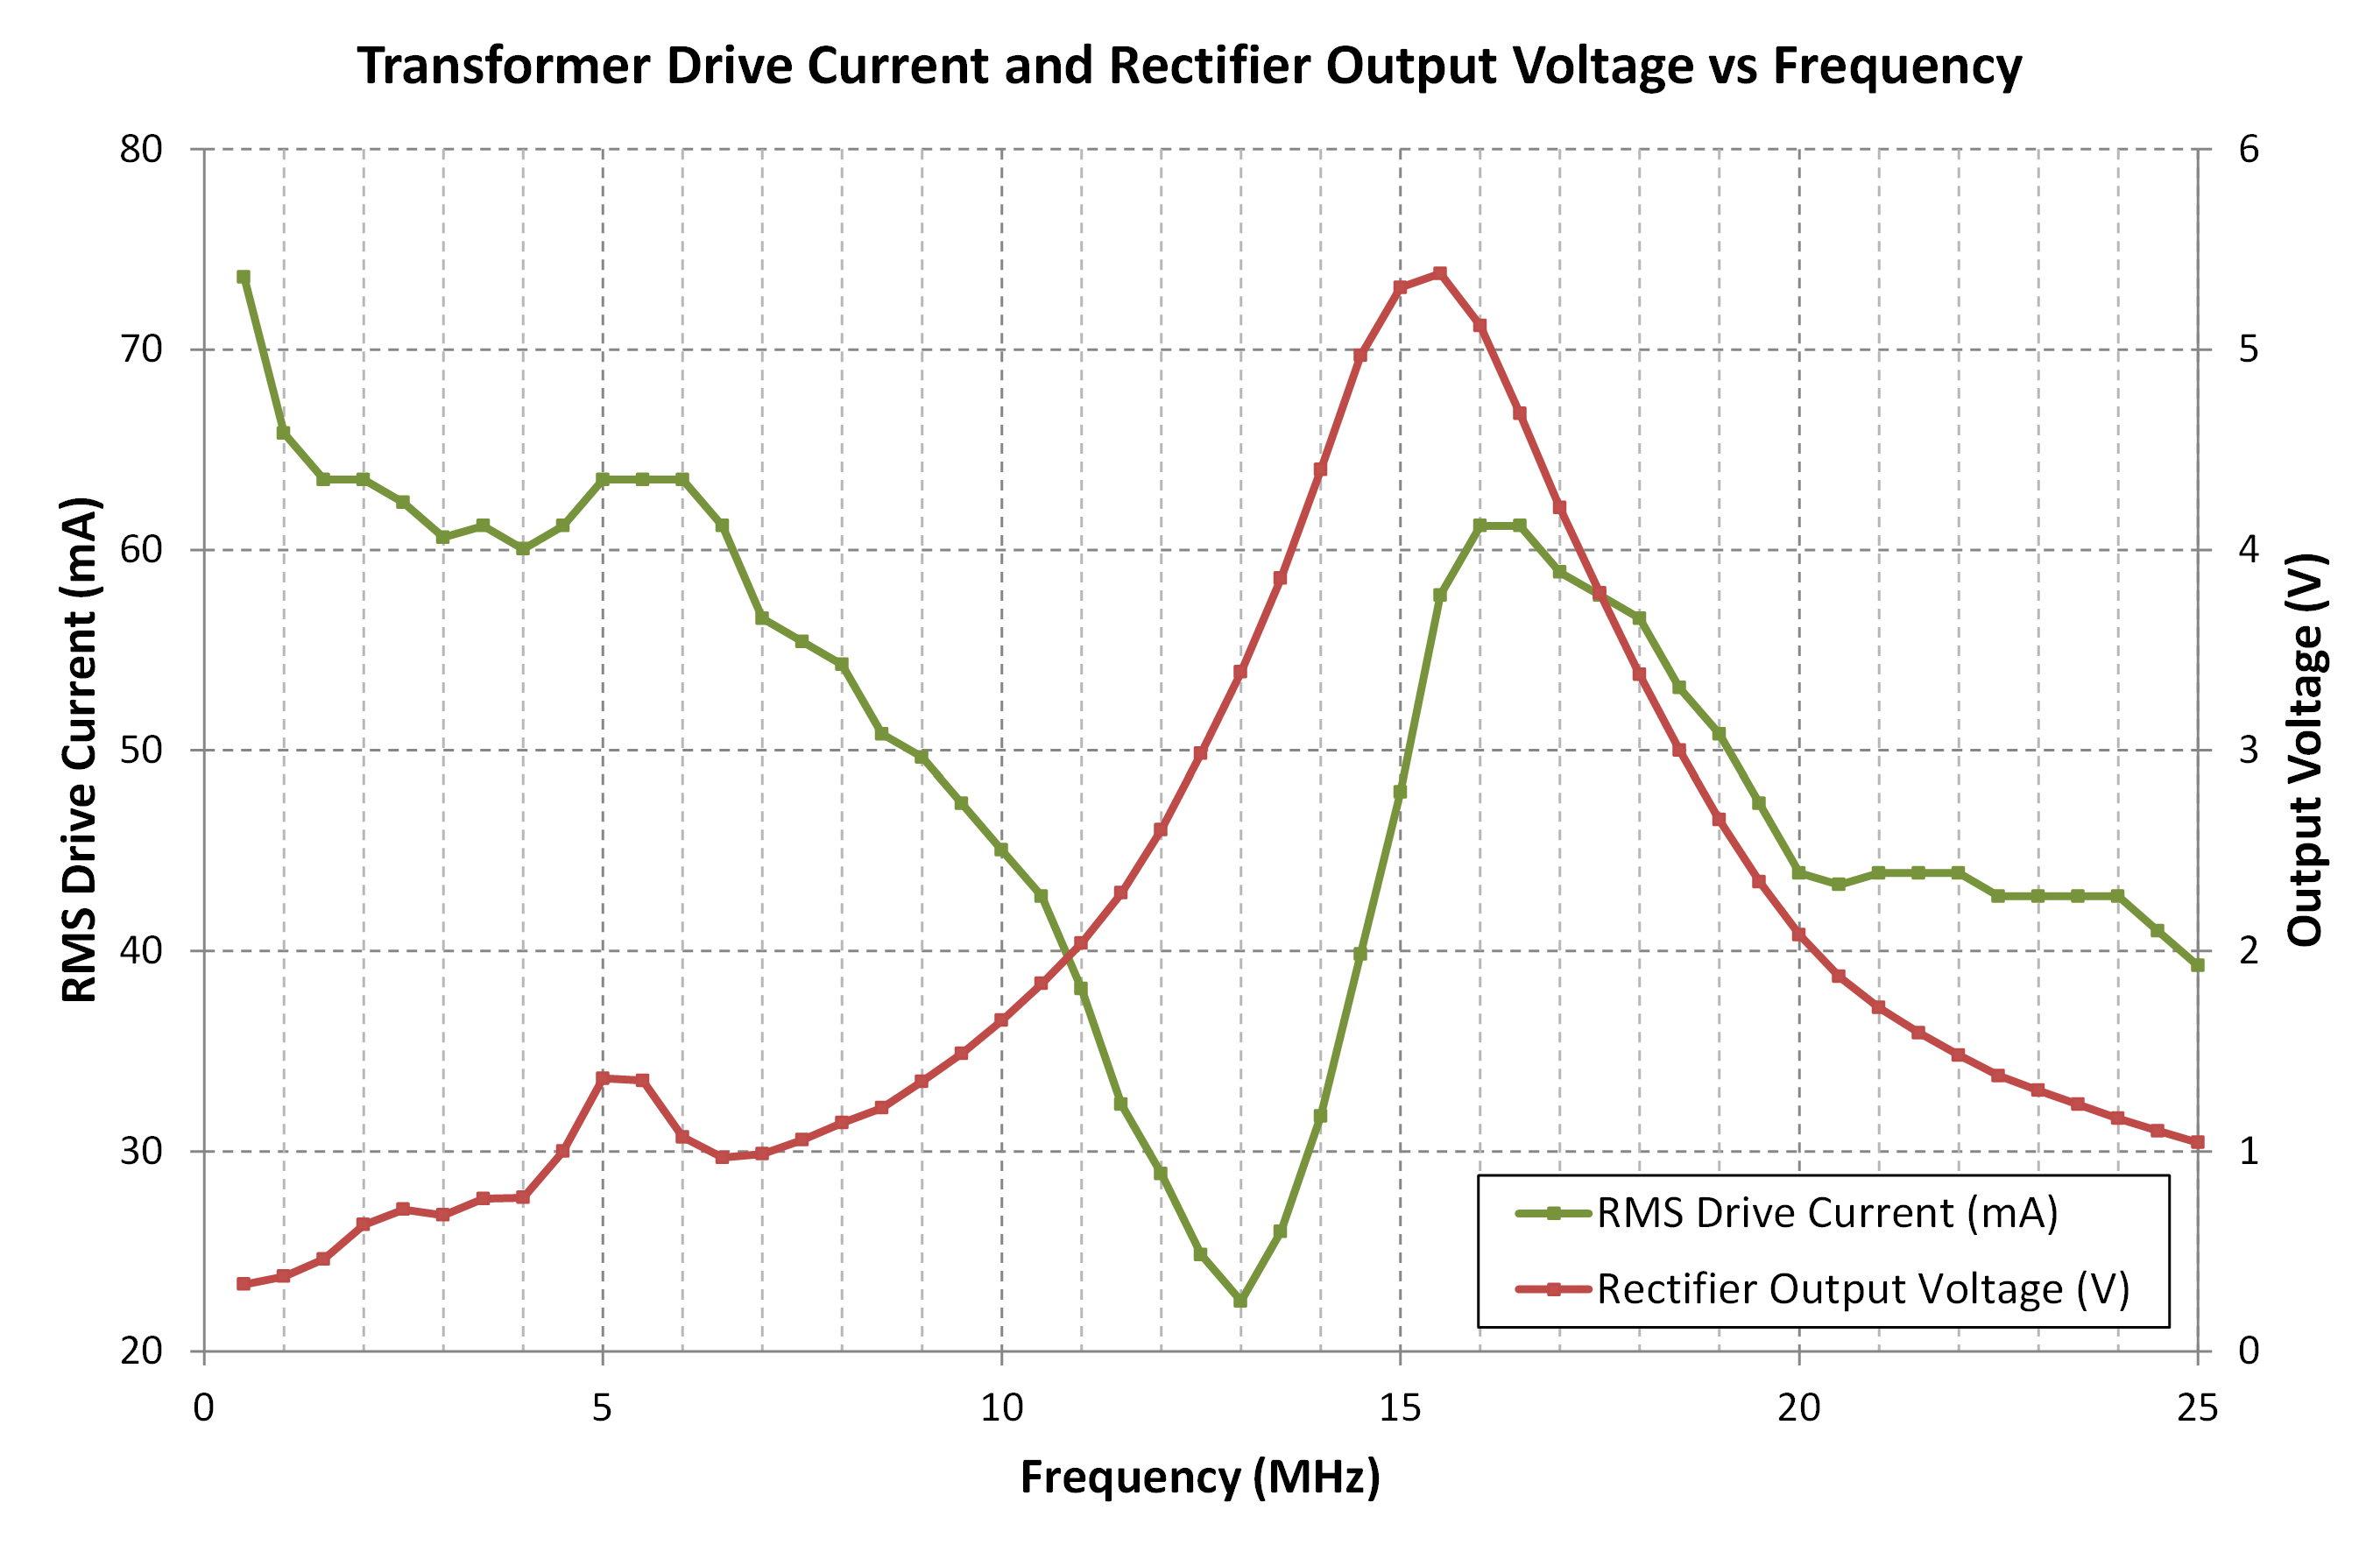
\includegraphics[width=1\columnwidth]{./img/ZandVoutVsF_3V3}
		\caption{Input impedance and output voltage versus frequency at 3.3V.}
		\label{fig:ZandVvsF}
	\end{figure}
	
	% MAHB: Reccomend putting these figures on the same horizontal scall so they are more easily compared. Figure text should be larger (nothing smaller than 8pt when scaled).
	\begin{figure}[t]
		\centering
		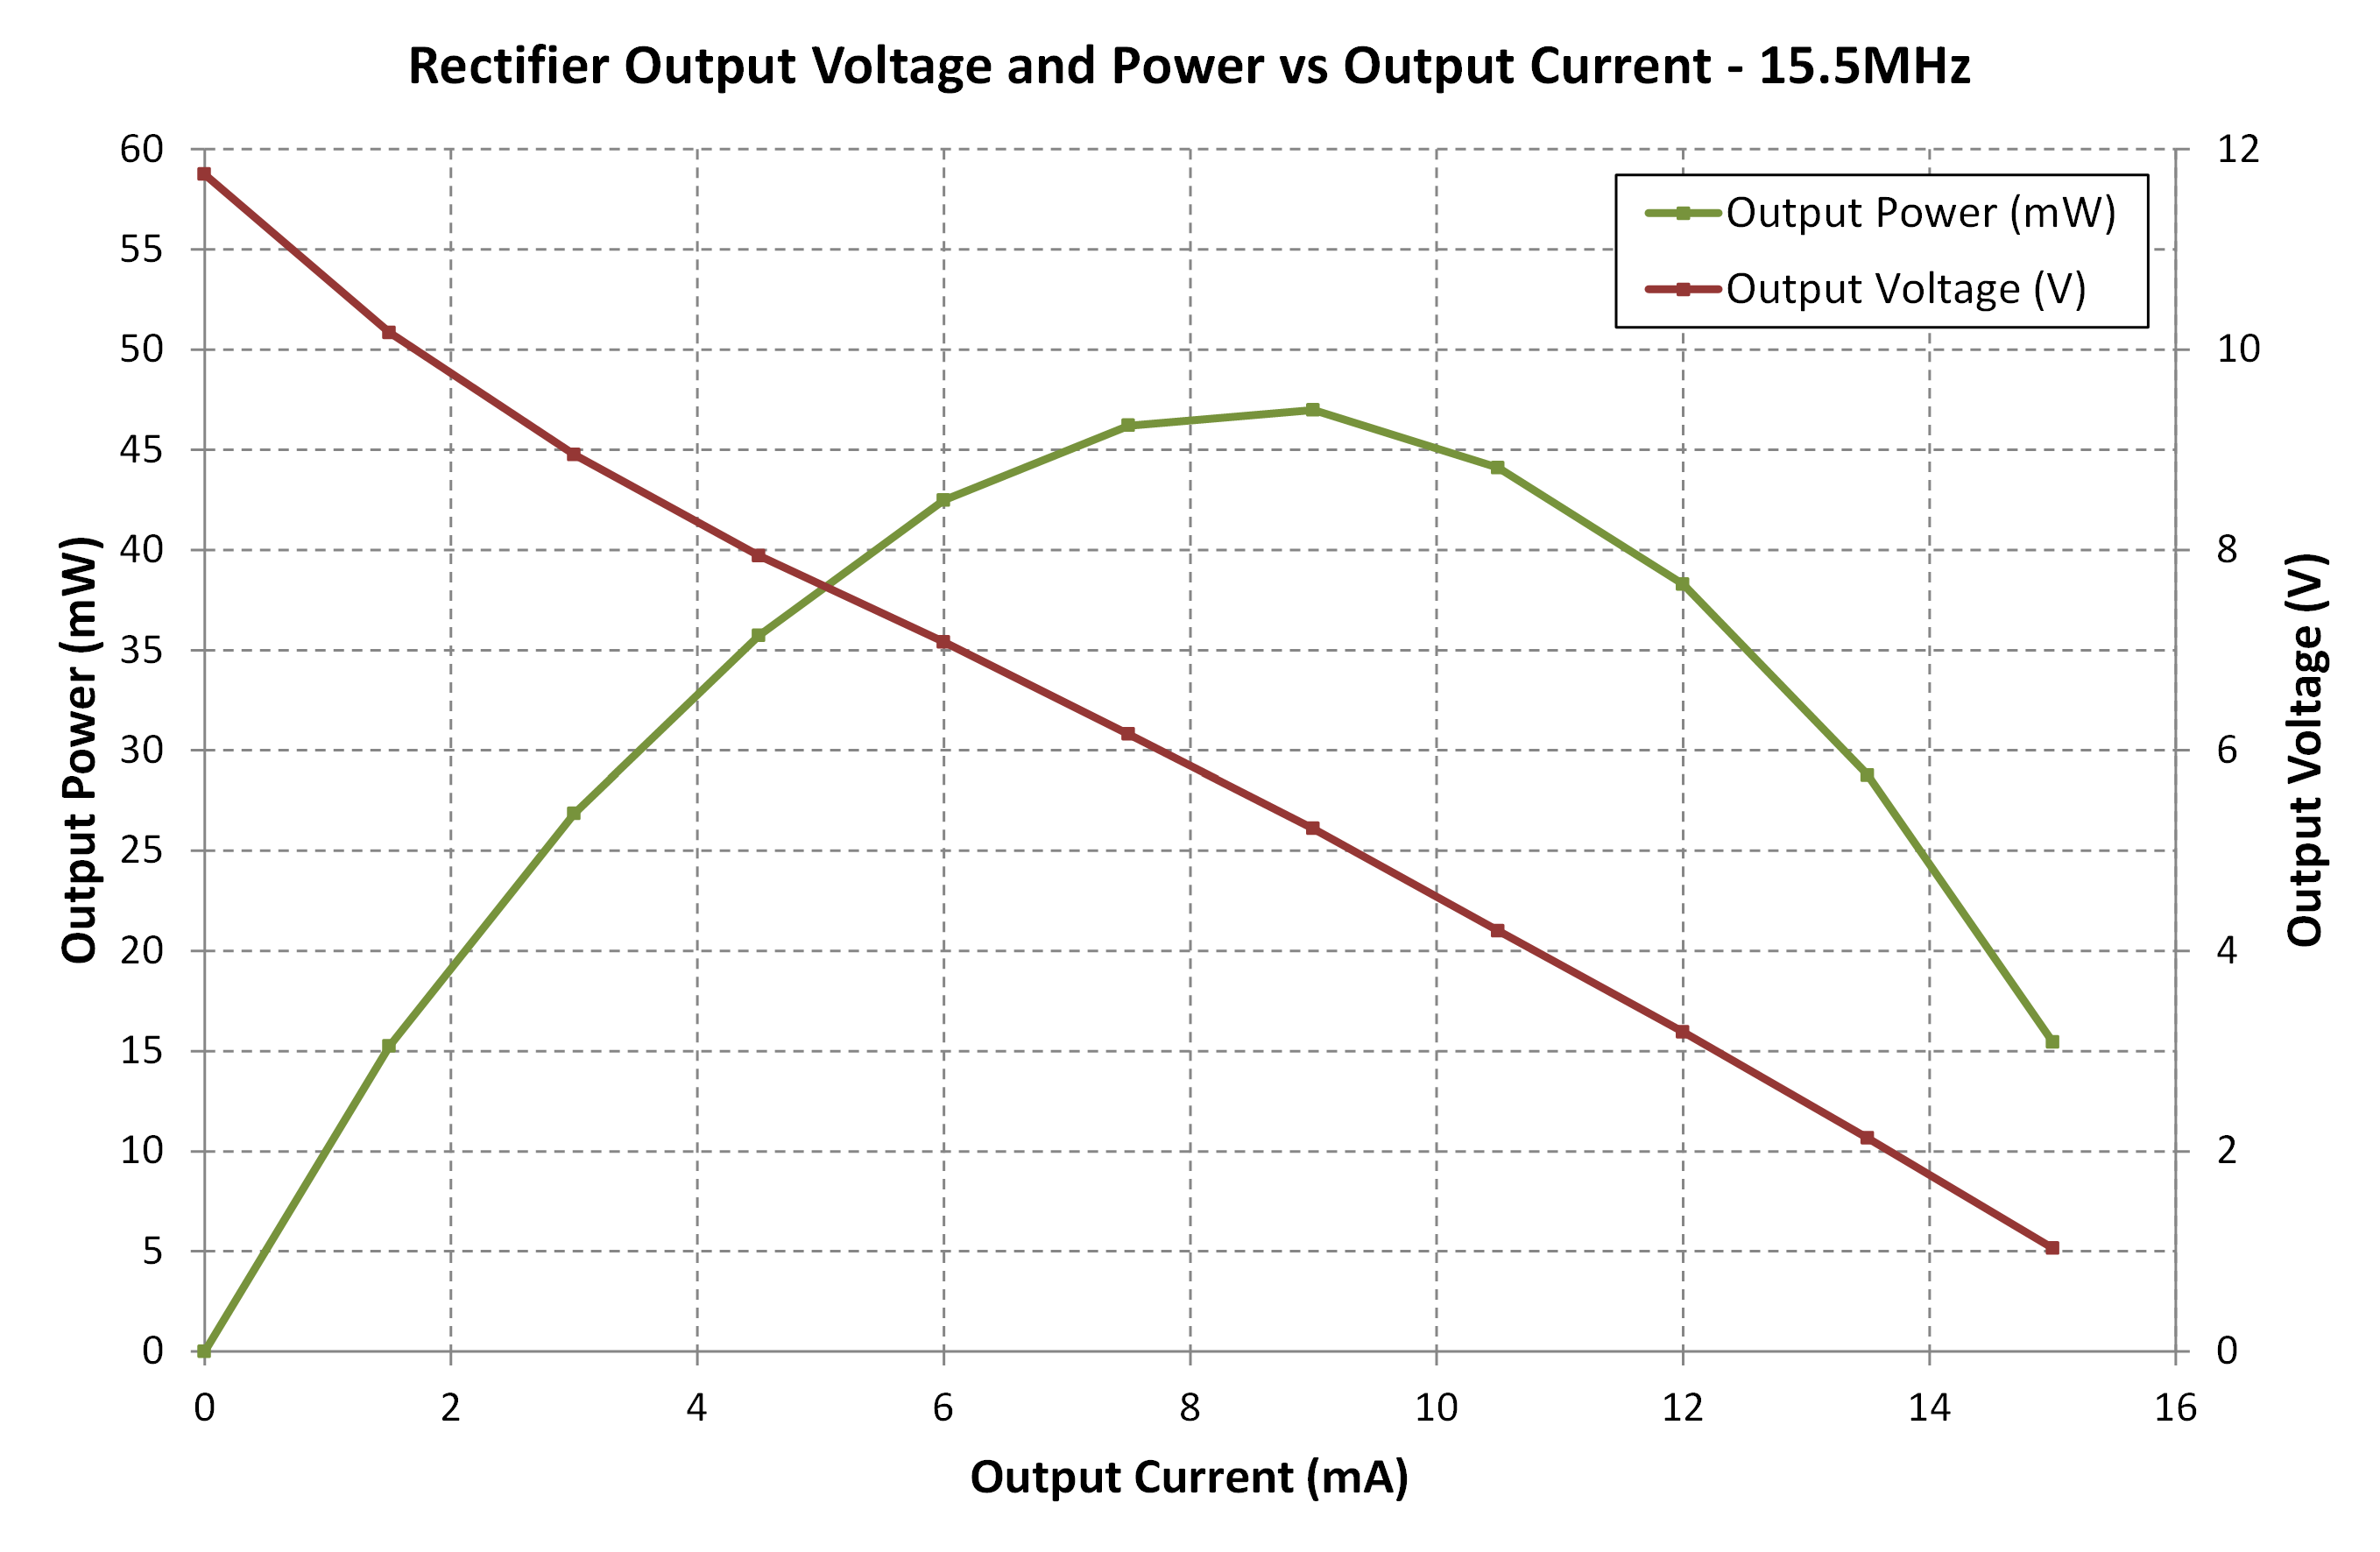
\includegraphics[width=1\columnwidth]{./img/VandPvsI}
		\caption{Secondary output voltage and power versus load current at MEF (15.5MHz).}
		\label{fig:VandPvsI}
	\end{figure}
	
	\begin{figure}[t]
		\centering
		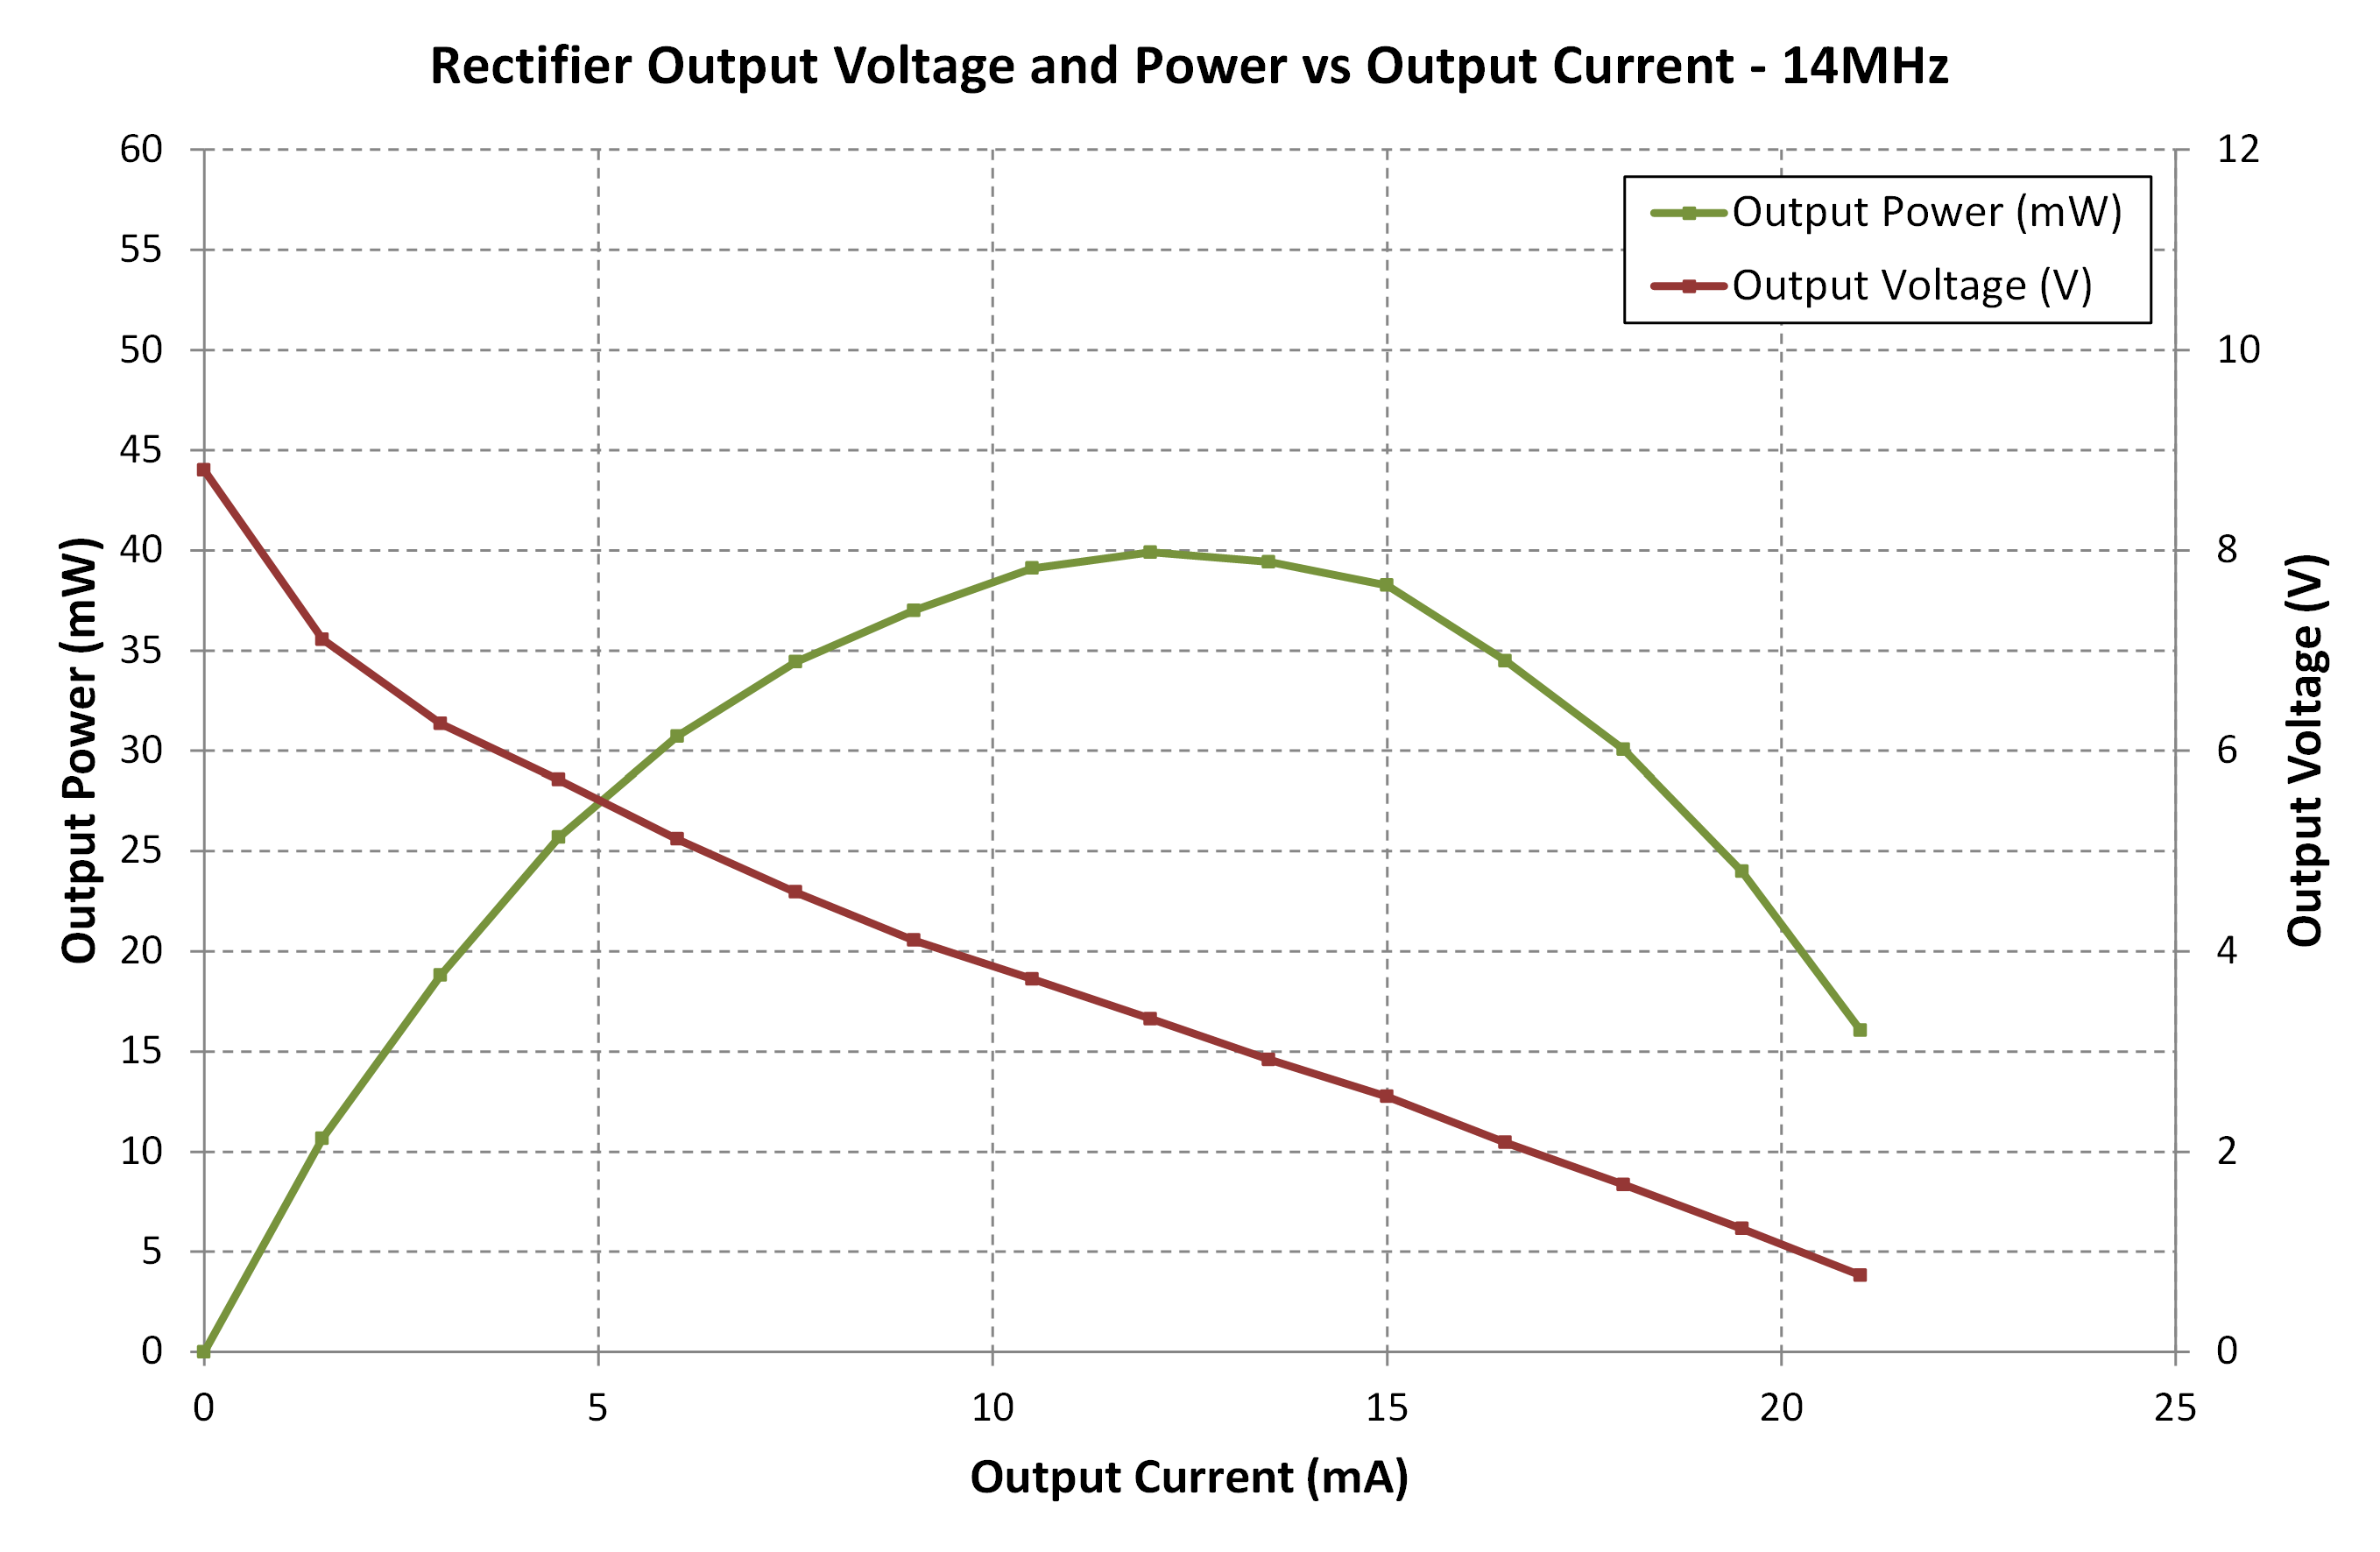
\includegraphics[width=1\columnwidth]{./img/VandPvsI_retuned}
		\caption{Secondary output voltage and power versus load current at MIF-MEF compromise (14MHz).}
		\label{fig:VanndPvsI_retuned}
	\end{figure}
	
	\subsection{Clock Generation and Recovery}
	Since the sigma-delta modulator's clock is derived from the drive frequency of the primary winding, it is necessary for the primary drive frequency to be an exact power-of-two multiple of the desired modulator frequency, which may vary from DC to 8MHz.  For the DAQM application, however, the external clock is necessary for multi-module synchronisation, and there is no desire to operate the sigma-delta modulator at a clock frequency other than 8MHz.  The test coreless PCB transformer has been designed for a 16MHz resonant frequency, with prior figures showing this to be the case in practice.  FIGURE shows the 16MHz clock signal (Reference - white), secondary output voltage (Channel 1 - yellow) and extracted clock signal (Channel 2 - cyan).  The divide-by-two clock extraction method appears effective, even with a varying secondary load, and further testing showed the simple circuit was able to accurately output a clock signal over the transformer drive frequency range of 11MHz to 16MHz.  The figures show no reason why a higher order division (divide by 4, for example) could not be used if desired.
	
	\begin{figure}[t]
		\centering
		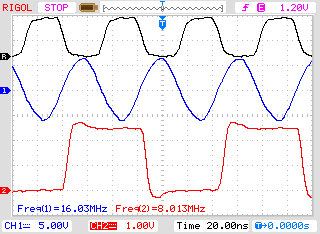
\includegraphics[width=0.8\columnwidth]{./img/Clock}
		\caption{16MHz input clock signal (top); secondary output voltage (centre); 8MHz extracted clock signal (bottom).}
		\label{fig:Clock}
	\end{figure}
	
	\subsection{Data Recovery}
	To test the data recovery circuit, a second PCB transformer was obtained with physical specifications identical to the unit discussed prior.  This second test transformer, however, had its load capacitor (which was 100pF in the prior unit) removed, such that its resonant frequency (now estimated to be $>$80MHz) was much greater than the expected data frequency - a key requirement of the data detection circuit.  Driving the transformer in a single-ended configuration was achieved by grounding one terminal and connecting the other, via a small capacitor, to a signal generator simulating the sigma-delta modulator's data output.  Due to hardware availability issues, the high-speed ($ t_{d} \leq 10ns $) Schmitt NAND gate specified in the circuit was substituted for an ordinary-speed ($ t_{d} \approx 250ns $) Schmitt NAND gate, which resulted in poor performance above about 500kHz (due to the fast impulses generated by the edge detection circuit).  FIGURE shows the data recovery circuit operating at 100kHz, where Channel 1 (bottom) is the 2MHz simulated data into the transformer; Channel 2 is the output of the negative edge amplifier (node `Neg Edge' in FIGURE); Channel 3 is the output of the positive edge amplifier (node `Pos Edge' in FIGURE); and Channel 4 (top) is the recovered 2MHz data signal.
	Since the data recovery circuit was capable of reliable operation with edge spikes of an amplitude as low as about 100mV, the 11-turn transformer was found to be excessive for the data signal transfer.  By cutting the PCB copper tracks on the primary and secondary side of the transformer, the performance of the data recovery circuit was tested for a transformer consisting of five turns and three turns.  The test showed that for a 3.3V square wave input, the five-turn and three-turn transformer yielded edge spikes of amplitude approximately 170mV and 50mV respectively.  FIGURE shows the positive and negative edge spikes at the secondary of the five-turn coreless PCB transformer with a 3.3V, 2MHz primary signal applied (via a small capacitor).  Testing has demonstrated that the data recovery circuit is effective over a range of data rates and duty cycles, and that a coreless PCB transformer with as few as four to five turns can be expected to yield reliable performance.
	
	\begin{figure}[t]
		\centering
		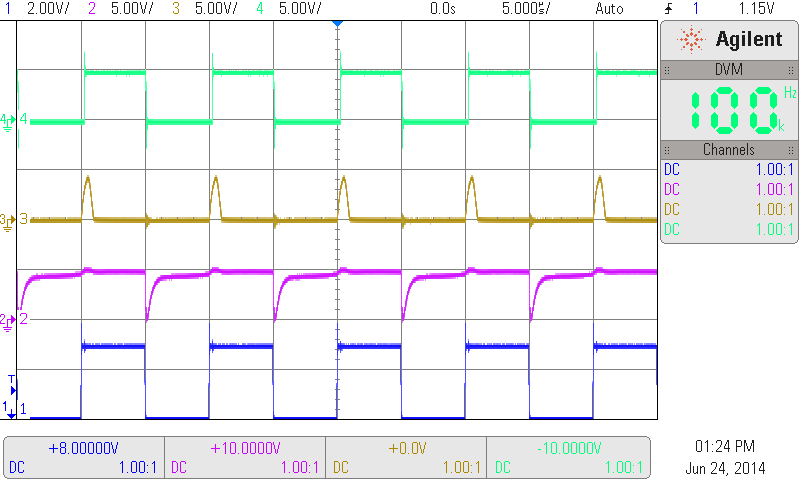
\includegraphics[width=0.8\columnwidth]{./img/DataUncropped}
		\caption{Data into transformer (CH1, bottom); output of negative edge amplifier (CH2); output of positive edge amplifier (CH3); recovered data signal at output of transformer (CH4, top).}
		\label{fig:Data}
	\end{figure}

	\begin{figure}[t]
		\centering
		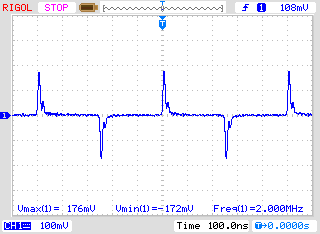
\includegraphics[width=0.8\columnwidth]{./img/5turnTF}
		\caption{Positive and negative edge spikes at secondary of 5-turn transformer (3.3V primary signal).}
		\label{fig:5turnTF}
	\end{figure}

% MAHB: Future work section would be a good idea. Discuss limitations of work to date.
\section{Future work}

\section{Conclusion}

Conclusion goes here.

% conference papers do not normally have an appendix	

% use section* for acknowledgement

% trigger a \newpage just before the given reference
% number - used to balance the columns on the last page
% adjust value as needed - may need to be readjusted if
% the document is modified later
%\IEEEtriggeratref{8}
% The "triggered" command can be changed if desired:
%\IEEEtriggercmd{\enlargethispage{-5in}}

% references section
\bibliographystyle{IEEEtran}
\bibliography{IEEEabrv,references}

\end{document}


